\documentclass[12pt, a4paper, oneside]{ctexbook}
\usepackage{amsmath, amsthm, amssymb, bm, graphicx, hyperref, mathrsfs}
\usepackage{geometry}
\usepackage{subfigure}
\usepackage{hyperref}[colorlinks=true,linkcolor=blue,citecolor=blue,urlcolor=blue,]
\usepackage{pdfpages}
\usepackage{svg}
\usepackage{url}
\usepackage{multirow}

\usepackage{multirow}
\usepackage{xcolor}[table,xcdraw]

%设置引用格式
\hypersetup{
	colorlinks=true,linkcolor=black,colorlinks=true,linkcolor=black,citecolor=blue,urlcolor=blue
}
%在LateX中,参考文献的引用一般有两种方式,平 齐 时 用 命 令\cite{...}, 上 标 时用\textsuperscript{\cite{...}}

\CTEXsetup[format={\Large\bfseries}]{section}	%section 居左(默认居中)
\CTEXsetup[format={\huge\bfseries}]{chapter}	%chapter 居左(默认居中)


%配置纸张边缘
\geometry{left=2.54cm,right=2.54cm,top=3.18cm,bottom=3.18cm}


\title{{\Huge{\textbf{FPGA验证文档}}}\normalsize{\\——第六届全国大学生集成电路创新创业大赛景嘉微杯初赛提交文档}}
\author{队名:虹ヶ咲学园芯片设计同好会\\ 成员:黄金源\space邓立唯\space林明锋}
\date{\today}
\linespread{1.5}


\begin{document}
	%-----------------------封面------------------
	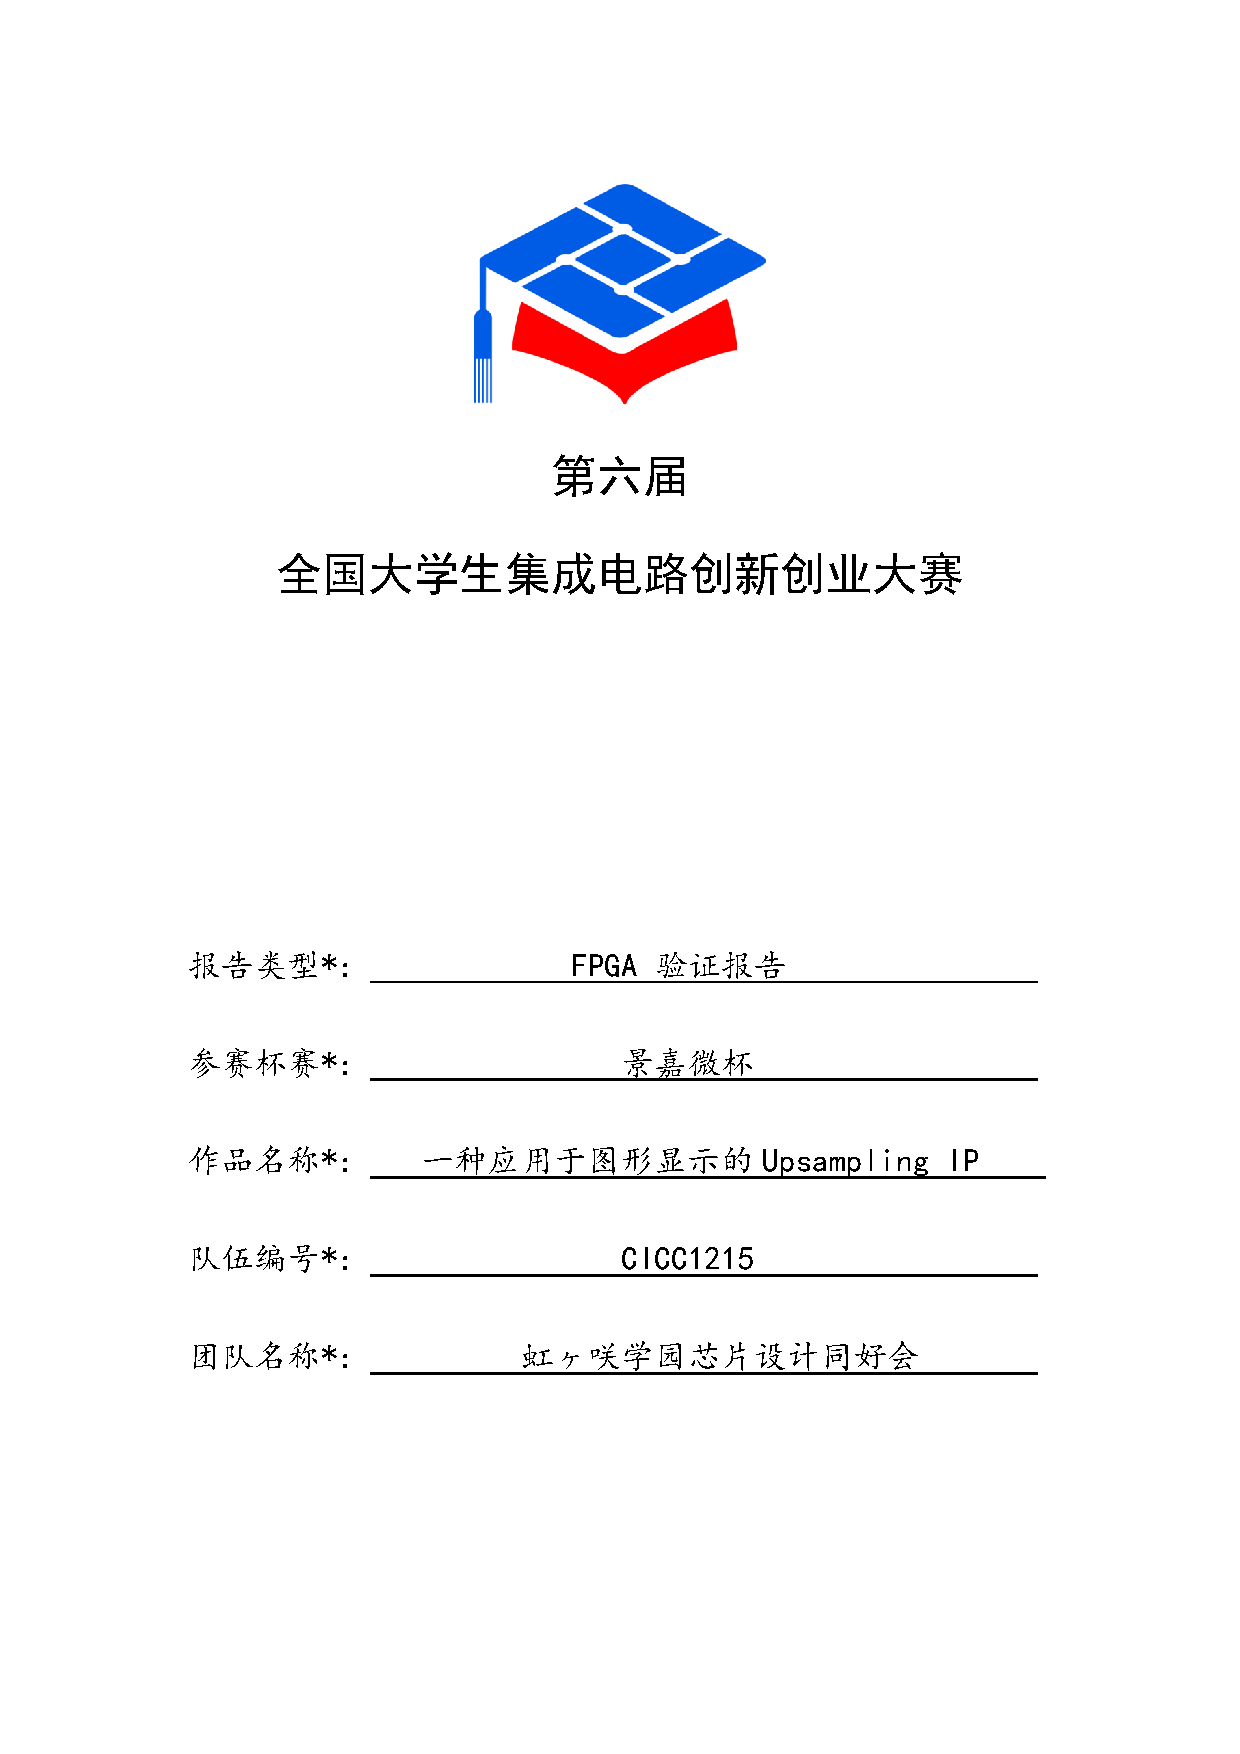
\includepdf{./pic/cover.pdf}
	\maketitle	
	\pagenumbering{Roman}
	\setcounter{page}{1}
	%-----------------------前言------------------
	\begin{center}
		\Huge\textbf{前言}
	\end{center}~\
	
	本文档(FPGA验证文档)仅作为虹ヶ咲学园芯片设计同好会(成员:黄金源、邓立唯、林明锋)参加第六届全国大学生集成电路创新创业大赛景嘉微杯赛初赛提交文档供评委评分使用。
	~\\
	\begin{flushright}
		\begin{tabular}{c}
			虹ヶ咲学园芯片设计同好会\\
			\today
		\end{tabular}
	\end{flushright}
	%-----------------------目录------------------
	\newpage
	\pagenumbering{Roman}	%Roman or arabic
	\setcounter{page}{1}
	\tableofcontents
	\newpage
	\setcounter{page}{1}
	\pagenumbering{arabic}
	
	%-----------------------正文----------------	
	\chapter{概述}
    在本项目中,需要进行 FPGA 板上验证的模块包括:Bicubic 上采样模块、纹理分类模块、自适应锐化模块。其中,已完成 FPGA 板上验证的有:Biubic 上采样模块;纹理分类模块与自适应锐化模块需要完成仿真验证后方可进行上板验证。
    \par
    关于 Bicubic 上采样模块具体验证方案可参考文档 \href{../../00 IP User Manual (All Specs)/APV21B_Bicubic_Super_Resolution_IP_UM.pdf}{APV21B-Bicubic Super Resolution IP User Manual} 第七章 Example Design。

    \chapter{验证方案}
    \section{验证平台介绍}
    本项目 FPGA 片上验证基于 米联客 MZU15A-15EG (Xilinx Zynq UltraScale+ MPSoC)完成。
    \section{验证框架介绍}
    验证框架参考文档 \href{../../00 IP User Manual (All Specs)/APV21B_Bicubic_Super_Resolution_IP_UM.pdf}{APV21B-Bicubic Super Resolution IP User Manual} 第七章 概述。
    \section{验证流程介绍}
    验证流程参考文档 \href{../../00 IP User Manual (All Specs)/APV21B_Bicubic_Super_Resolution_IP_UM.pdf}{APV21B-Bicubic Super Resolution IP User Manual} 第七章 设计工作流程。
    \begin{figure}[t]
        \centering
        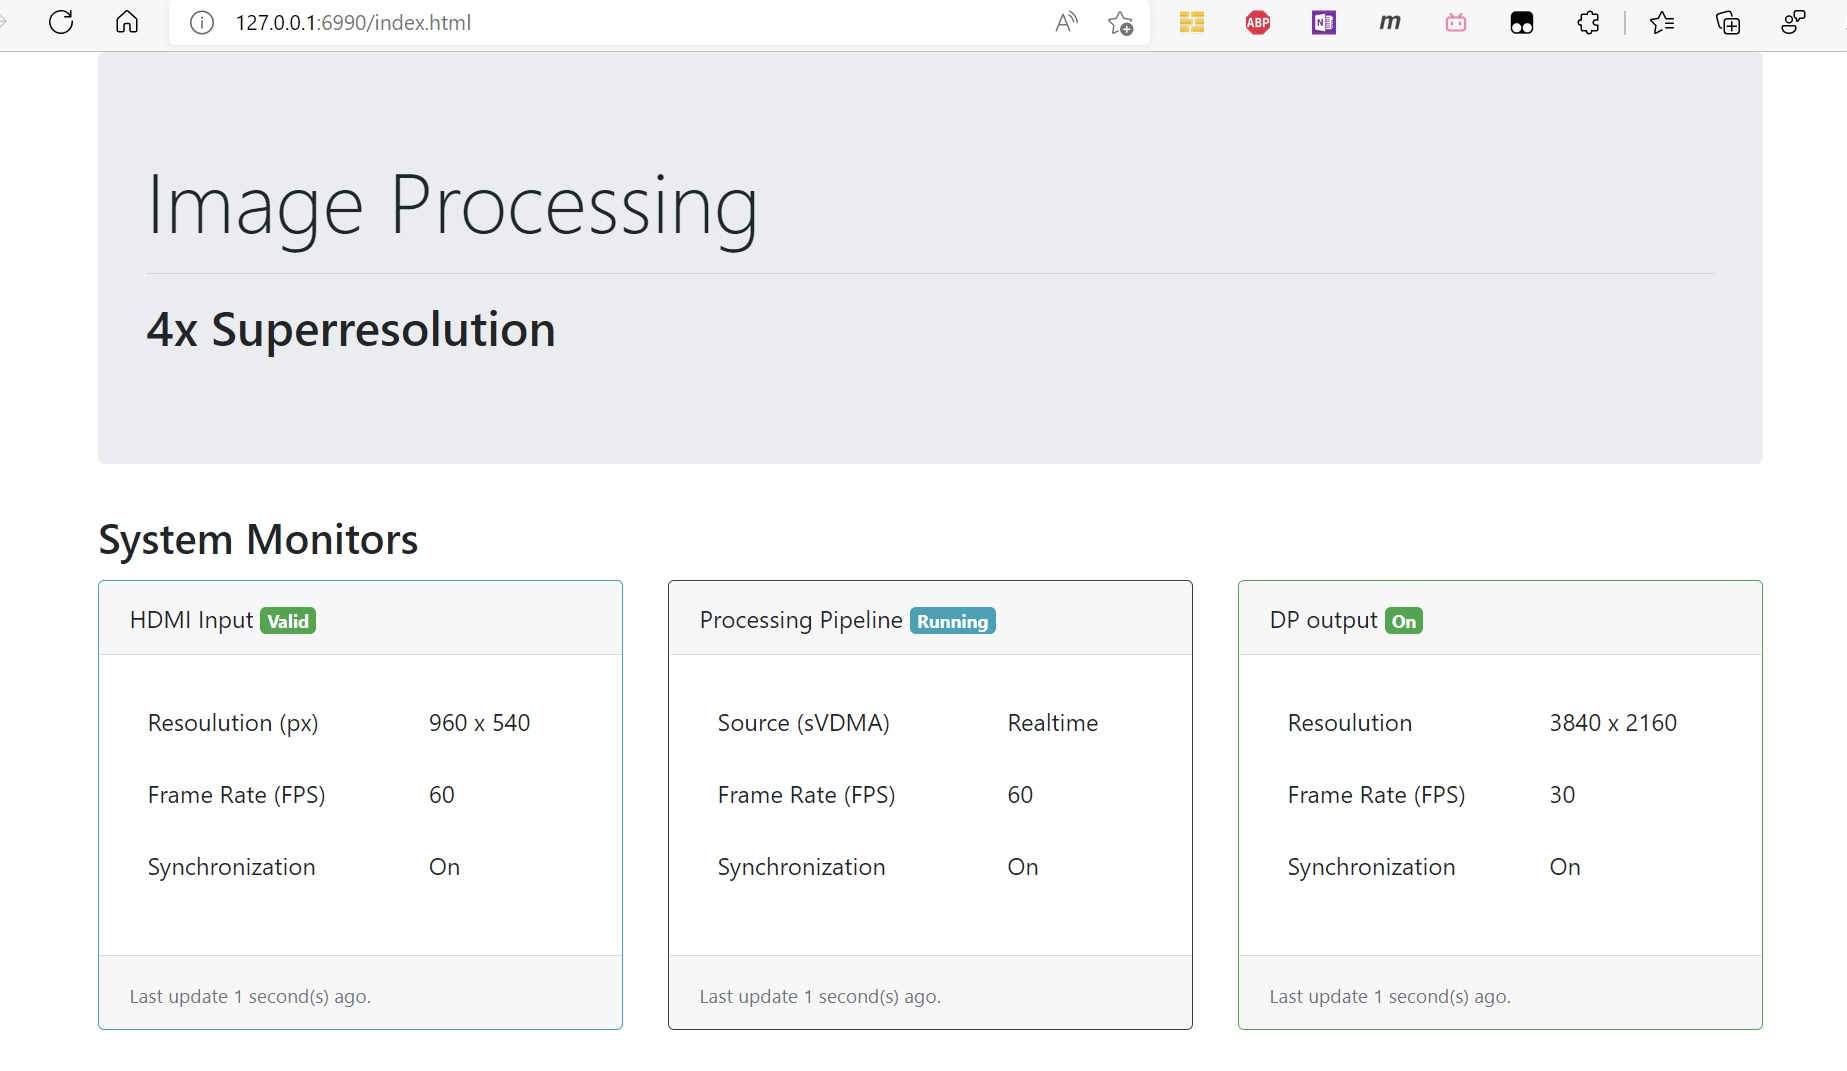
\includegraphics[scale=0.2]{pic/web.jpg}
        \caption{上位机界面展示}
        \label{web}
    \end{figure}
    \section{上位机介绍}
    基于 Bootstrap 前端框架,使用 JavaScript 和 CSS 开发了网页端上位机,本地主机或服务器通过千兆以太网与 FPGA 开发板 PS 侧连接,可实现实时图像、视频数据、控制指令交互功能。页面如 \ref{web} 显示。
    
    \newpage
    \subsection{输入模式选择}
    \begin{itemize}
        \item HDMI 实时输入
        \item 网页上传图片
    \end{itemize}
    \subsection{其他功能}
    \begin{itemize}
        \item 实时状态监视
        \item 网页控制(一键)处理流程
        \item 自动将处理好的图片并打包成 ZIP 并保存
    \end{itemize}

    
	

\end{document}
